\ifgerman{\chapter{Grundlagen}}{\chapter{Background and Related Work}}
\label{background}
This chapter is structured to provide readers detailed insights of fundamental information required to understand this thesis. \ref{section: document matching} presents the bedrock concepts about document matching, applications and their necessity in the present world. In \ref{section: rcv1}, we provide a glimpse of our input dataset structure and its statistics. The process of document matching and its in-detail insights are illustrated in \ref{section: process of document matching}. Later, a brief introduction to  MapReduce and its limitations are discussed in \ref{section: Mapreduce}. In \ref{section: apache spark}, the concepts of Apache Spark framework that includes insights from basics to in-detail explanations of the ecosystem are emphasized. In \ref{section: Related work}, we discuss the previously implemented related work in the areas of document matching and Latent Dirichlet Allocation (LDA).

\section{Document Matching}
\label{section: document matching}
In the present realm of web-based and cloud-based technologies, the volume of the documents ranging from world wide web (WWW), online forums, digital libraries to news articles is increasing at rapid pace. On one hand processing this magnitude of documents efficiently is a challenging task and on the other hand, matching these documents by means of semantics would be of much more greater scale. 


\par  A corpus is a large collection of documents. In corpus based similarity, semantic similarity is carried out by measuring the similarity between documents with the help of information attained from the large corpora \cite{gomaa2013survey}. Within a Corpus, the problem of extracting similar documents based on their semantics has been broadly addressed by information retrieval community.

\par A subset of such addressing is based on the extraction of feature vectors from documents. The process starts by extracting feature vectors (words) from documents and then weighted by means of term frequencies (TF-IDF) which in turn produces a sparse vector and ends by comparing the documents in these sparse distances. But there are two problems associated with this process, one is the representation of feature vectors as sparse vectors. As these sparse vectors can be high dimensional which may require greater computational power. Additionally, the size of the feature vector increases with increase in the length of the document. Hence the approach is appreciable for fixed length document. The other is that the TF-IDF approach is reliable on only word occurrences which may not give desirable results if two documents are having the same context but are expressed with different representations or different words. For Example, consider the following two news articles published by two different newsgroups :
\newline

Article 1: A gigantic cyclone hit the southern part of Germany. 
\newline
\par Article 2: Eventually, part of Germany was stormed by the hurricane on a massive scale.
\newline
\par From the above two articles, we can observe that the two articles are speaking about the same information contextually but expressed in different terms. This is the major limitation of any approach that uses TF-IDF though the problem of high dimensionality is addressed by various dimensionality reduction algorithms. 

\par We try to describe an implementation which involves in addressing the above stated problems such as match documents irrespective of its contained length. Instead of just relying on word occurrences, our implementation additionally considers the structure of the document. Also, we implemented our application using the parallel environment to process a huge volume of documents as our primary focus is on reducing execution time and are discussed in consecutive sections.


\subsection{Applications}
In this section, some of the examples that are used for document matching application are illustrated in the following:

\begin{itemize}
\item \textbf{Help Desk Application:} Help-desk in any institute or organization plays a vital role in helping their customers or users. The application is implemented to act as a response system. The focus of the application is to help its users to provide necessary information on problem description. A user has to input a problem description and the application takes that problem as a query and is compared to the entire corpus in order to provide the useful information to the user. For this purpose, document matching techniques are used \cite{weiss2000lightweight}.

\item \textbf{Literature Search Tool:} PubMed is a literature search tool developed by National Center for Biotechnology Information at United States National Library of Medicine. The literature consisting of over 28 million citations. The tool provides results based on the keywords provided to the query. The available literature covers a range of biomedical, health, chemical sciences, bioengineering to life sciences. For any given query, the search engine of the PubMed tool produces results based on the document pair similarity scores \cite{website:pubmed}. 
\end{itemize}


\newpage
\section{Reuters Corpus Version 1}
\label{section: rcv1}

\begin{figure}[hp]
	\centering
		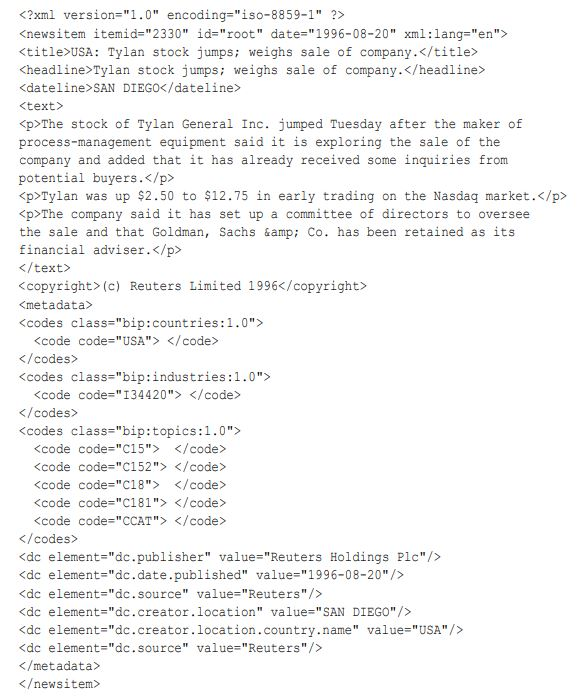
\includegraphics[scale=1.00]{Reutersdoc}
	\caption{A sample document from Reuters Corpus Version 1 \cite{lewis2004rcv1}}
	\label{fig:reutersdoc}
\end{figure}

The dataset that we used as input is Reuters Corpus Version 1 (rcv1). Rcv1 in total has 806,791 documents that are manually categorized news articles from Reuters Ltd. The contents of all the documents are in the English language. From the \ref{fig:reutersdoc}, it can be seen that the documents are produced in extensible Markup Language (XML) format and provides further sophisticated information about how a document is produced. The additional information about the corpus and document structure are discussed in the following \cite{lewis2004rcv1}:
\begin{itemize}
\item Every document consists of unique document ID and range from 2286 to 810597. In \ref{fig:reutersdoc}, the document id can be found as itemid in between the tags named newsitem. This unique Document ID is used for the entire document matching process.

\item From \ref{fig:reutersdoc}, the data in between the tags named text is the news article that is providing information about the specific context where <p> represents a paragraph. The whole data in between text is required for the process of document matching.  

\item  All the documents in the corpus are divided into three categories namely Topics, Industries, and Regions.

\item A total of 103 codes are available under topics and the assignment of the topic to a document is performed within these codes. A document can have no assignment, a single assignment or multiple assignments of codes. The assignment of codes was performed automatically but under the supervision of human editors. In \ref{fig:reutersdoc}, the assignment of the various topics to a single document can be seen in between the tags codes that point to the class bip:topics:1.0

\item The document also provides an additional metadata information such as copyright that a document belongs to, the origin of document or news article generated, the date that news article published etc.
\end{itemize}
  
\par For evaluation purposes, We have chosen Reuters corpus as we need a large amount of documents in order to evaluate the parallel performance and scalability of our application. The corpus does not possess any information or labels that represent the semantic relation between two documents which can be in short called as the ground truth table. Hence we have implemented a work around method to generate gold standard data and is used for effectiveness evaluations. The detail description of the workaround method is discussed in \ref{implement:evaluation}.


\section{Process of Document Matching}
\label{section: process of document matching}

\begin{figure}[htp]
	\centering
		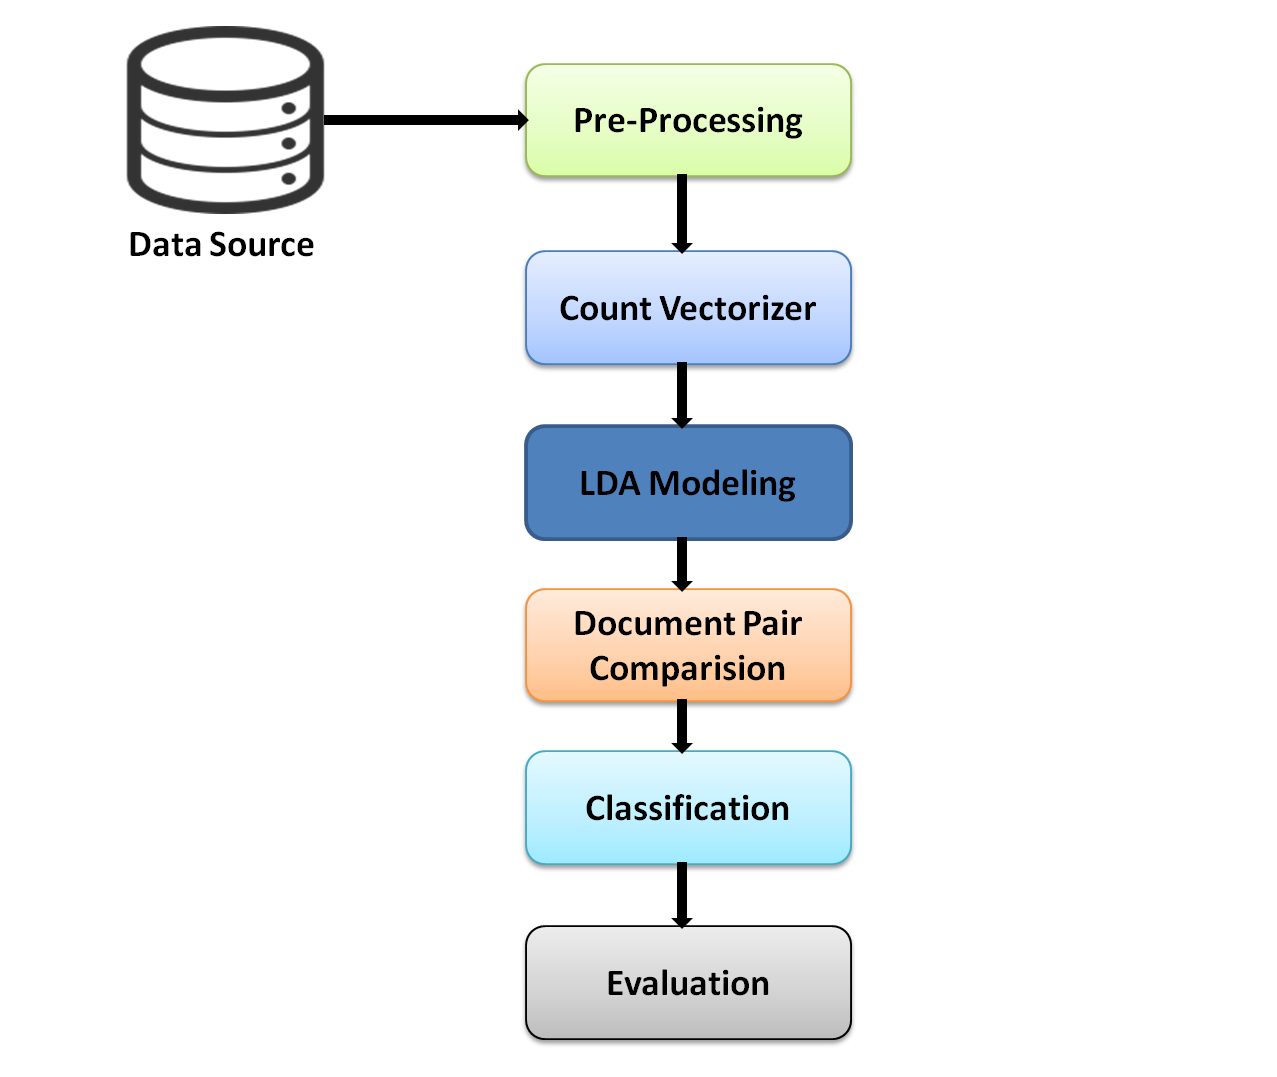
\includegraphics[scale=0.60]{Process}
	\caption{Work flow of Document matching process}
	\label{fig:process}
\end{figure}

As illustrated in the \ref{fig:process}, the implementation of the Document Matching involves six major stages namely pre-processing, count vectorization, Modeling, Document pair comparison, Classification, and Evaluation. The detailed information provided in the following sections improves ones understanding of the document matching process. \ref{section: preprocessing} provides information on the requirement of a pre-processing stage. A document is required to be represented in sparse vectors for any algorithm to understand and are discussed in detail in \ref{section: countvectorizer}. Once a document is represented in a sparse vector, it is then sent to document modeling algorithm for the purpose of document matching and \ref{section: lda} provides detailed insights. To find which documents are matching semantically, every document in the corpus is compared to other document and the logical theory behind it is discussed in \ref{section: document pair comparison}. In the classification stage, the compared documents are classified as match or non-match and the classification techniques used for the purpose are explained in \ref{section: classification}. Finally, the output from the classification stage is sent to the last stage called evaluation stage where certain evaluation schemes are used and are elucidated in \ref{section: evaluation}.


\subsection{Pre-processing}
\label{section: preprocessing}
The first step of our implementation is pre-processing of data. As can be seen from \ref{fig:reutersdoc}, the data which we require is a document and is in XML structure and has to be cleaned and to be brought to a data format that is acceptable by the framework before initializing to any further steps. It is essential to filter out unwanted data otherwise it may lead to inaccurate computations which may finally results in inaccurate evaluations. Hence, it is mandatory to clean the data in order to increase the input data quality. Internally, this step is further divided into three phases consisting of parsing data, tokenization and stop words removal and are explained in the following:
\begin{enumerate}
\item \textbf{Parsing Data:} If the data is semi-structured and holds different kinds of information in the same document. It is required to separate and retrieve the relevant data fields from the irrelevant ones.

\item \textbf{Inferring Schema:} After the required data fields are extracted from the document, then we have to standardize the data fields according to the acceptable data format either by inferring schema implicitly or explicitly.

\item \textbf{Tokenizaton:} The process of breaking or splitting a sentence to a series of individual words is referred as tokenization. The individual words generated in this process can be called tokens. It is also obligatory to remove special characters such as `,' , `<' ,`\' , `?' etc as these characters do not possess any useful information in the process of document matching.

\par For example, let us consider two sentences and observe how a tokenization process extract tokens and is illustrated in \ref{tab:tokenization process example}.

\begin{table}[htbp]
	\centering
		\begin{tabular}{ccc}\toprule
			& Input & Output\\\midrule
		Sentence 1 & Hello! < how are you?> & [ hello, how, are, you ]\\\addlinespace 
		Sentence 2 &  I love to travel countries & [ i, love, to, travel, countries ] \\\addlinespace
			\bottomrule
		\end{tabular}
	\caption{An Example of tokenization process}
	\label{tab:tokenization process example}
\end{table}



\item \textbf{Stop Words Removal:} The words that frequently appear in the data and doesn't hold neither useful information nor influence of meaning on the document is referred as stop words \cite{fox1989stop}. Some of the stop words include I, the, is, a etc. As these words have no significance, these words are to be removed from the data.

\par An example is illustrated in \ref{tab:stopwords process example}.

\begin{table}[htbp]
	\centering
		\begin{tabular}{ccc}\toprule
			& Input & Output\\\midrule
		Sentence 1 & The dog is a good pet & [ dog, good, pet ]\\\addlinespace 
		Sentence 2 &  I wish  to travel the world & [ wish, travel, world ] \\\addlinespace
			\bottomrule
		\end{tabular}
	\caption{An Example of stop words removal process}
	\label{tab:stopwords process example}
\end{table}


\end{enumerate}


\subsection{Count Vectorizer}
\label{section: countvectorizer}
In our application, after cleaning of the input data, A document has to be converted to vector representation for further processing and can be performed using Count Vectorizer. The numerical values generated inside the vector by Count Vectorizer represents the influence of a single word that has with the particular document in the Corpus. Count Vectorizer builds a matrix that is sparse in nature based on the word occurrence of each document in the corpus. The matrix consists of documents over Vocabulary. Count Vectorizer maintains a dictionary in which the unique words are stored and compared.  For example, we presume that we have four different documents containing respective sentences as illustrated in  \ref{tab:documents and sentences}.

\begin{table}[htbp]
	\centering
		\begin{tabular}{cc}\toprule
			Document & Sentence\\\midrule
			1 & Hello How are you\\\addlinespace 
			2 &  How do you do\\\addlinespace
			3 & Where are you\\\addlinespace
            4 & Where you been\\\addlinespace
			\bottomrule
		\end{tabular}
	\caption{Documents containing sentences}
	\label{tab:documents and sentences}
\end{table}

\par Firstly the process of Count Vectorizer starts by creating a dictionary of unique words that it recognizes from documents. An unique ID is assigned to every unique word and the dictionary for documents \ref{tab:documents and sentences} is illustrated in \ref{tab:dictionary}.

\begin{table}[htbp]
	\centering
		\begin{tabular}{cc}\toprule
			ID & Word\\\midrule
			1 & Hello \\\addlinespace 
			2 &  How  \\\addlinespace
			3 & are\\\addlinespace
            4 & you \\\addlinespace
            5 & do \\\addlinespace
            6 & Where \\\addlinespace
            7 & been \\\addlinespace
			\bottomrule
		\end{tabular}
	\caption{Dictionary by Count Vectorizer }
	\label{tab:dictionary}
\end{table}

\par The dictionary in \ref{tab:dictionary} represents that a total of seven distinct words found by the Count Vectorizer for four documents respectively.

\par Now by considering the dictionary, the Count Vectorizer generates a matrix by mapping the presence of feature along with times the feature appeared in that particular document as shown in \ref{tab:Document vocabulary Matrix}. From the \ref{tab:Document vocabulary Matrix}, we can observe that every 1 represents the occurrence of a feature that appeared in the particular documents whereas 0 states the absence of that particular feature in that document. The count of the particular feature is proportional to the number of times the feature appears in the particular documents and the same can be observed within document 3.


\begin{table}[htbp]
	\centering
		\begin{tabular}{cccccccc}\toprule\addlinespace
			 & Feature 1 & Feature 2 & Feature 3 & Feature 4 & Feature 5 & Feature 6 & Feature 7\\\addlinespace\midrule
			Document 1 & 1 & 1 & 1 & 1 & 0 & 0 & 0 \\\addlinespace
       
			Document 2 &  0 & 1 & 0 & 1 & 2 & 0 & 0 \\\addlinespace
            
			Document 3 & 0 & 0 & 1 & 1 & 0 & 1 & 0\\\addlinespace
            
            Document 4 & 0 & 0 & 0 & 1 & 0 & 1 & 1\\
            \bottomrule
		\end{tabular}
	\caption{Document Vocabulary Matrix  generated by scheme of Count Vectorizer}
	\label{tab:Document vocabulary Matrix}
\end{table}

\par The final representation of the sparse vector generated by Count Vectorizer can be seen in \ref{tab:vector representation} where 7 represents the dictionary size, the second array represents the IDs of the appeared features in the particular document and third array represents the word occurrences of the particular feature.


\begin{table}[htbp]
	\centering
		\begin{tabular}{cc}\toprule
			  & Vector\\\midrule
		Document 1 & (7, [1,2,3,4], [1,1,1,1])\\\addlinespace 
		Document 2 &  (7, [2,4,5], [1,1,2])\\\addlinespace
		Document 3 & (7, [3,4,6], [1,1,1])\\\addlinespace
        Document 4 & (7, [4,6,7], [1,1,1])\\\addlinespace
			\bottomrule
		\end{tabular}
	\caption{Vector representation by Count Vectorizer}
	\label{tab:vector representation}
\end{table}

\subsection{Latent Dirichlet Allocation}
\label{section: lda}
This step is the heart of our application. It aims at building a document-topic matrix based on how a document can be expressed in terms of its context and is discussed in detail in the following.

\begin{figure}[htbp]
	\centering
		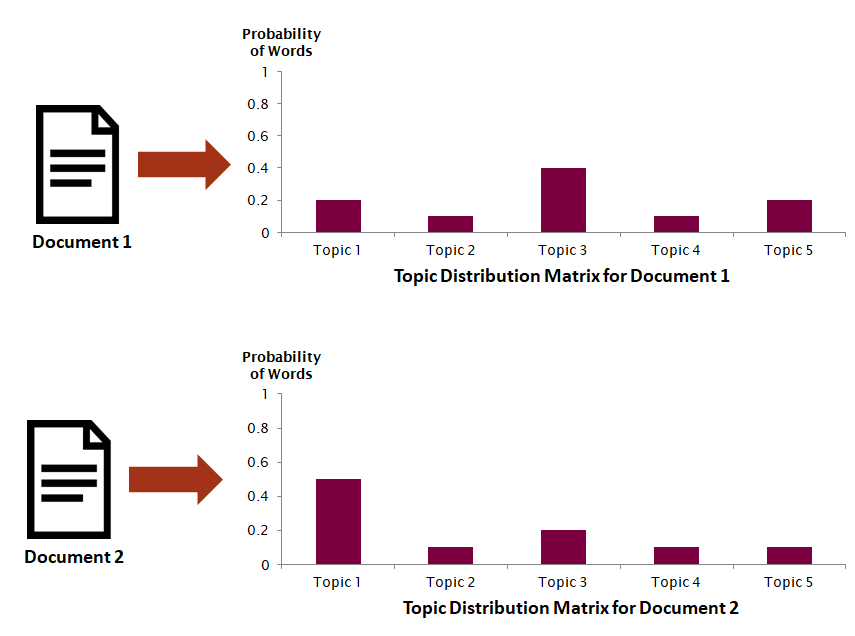
\includegraphics[scale=0.65]{lda}
	\caption{Representation of a sample documents in terms of 5 topics by Latent Dirichlet Allocation }
	\label{fig:lda}
\end{figure}

\par In 2003,  researchers David M. Blei, Andrew Y.Ng and, Michael I. Jordan first proposed a topic modeling algorithm for a large set of text documents referred as Latent Dirichlet Allocation (LDA). LDA is an unsupervised machine learning algorithm. LDA can also be used for context visualization and context summarization on huge voluminous document collections.  As illustrated in \ref{fig:lda}, LDA represents a document as a probabilistic distribution of topics where the axis named probability of words represents the total number of words contributing to the particular topic \cite{blei2003latent}. From \ref{fig:lda}, we can observe the different topic distributions for different documents.


\par LDA assumes that a document is produced or written with the following criteria:
\begin{itemize}
\item Every document is a probabilistic distribution of topics
\item Every topic is a probabilistic distribution of words
\end{itemize}

\par Based on the above assumptions, LDA observes the words in any given document and assigns a probability to each word that belongs to a topic finally resulting in topic distribution and can be seen in \ref{fig:ldacorpus}.
\begin{figure}[htbp]
	\centering
		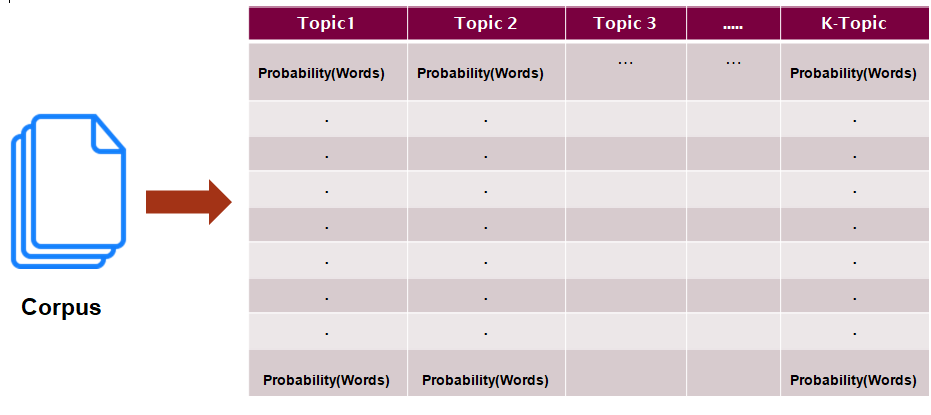
\includegraphics[scale=0.60]{ldacorpus}
	\caption{Representation of a corpus in terms of document topic matrix by Latent Dirichlet Allocation where each row of the matrix represents a document}
	\label{fig:ldacorpus}
\end{figure}


\par From \ref{fig:ldacorpus}, a corpus is a collection of the large set of documents. Each row represents a document and is represented by K latent topics. By this matrix, any two documents can be compared to calculate the semantic similarity between them as the documents are representing the structure or context. 

\par We have used the following learning algorithm for LDA to discover the topics and is discussed:

\textbf{Expectation Maximization:} 

Expectation Maximization algorithm contains two steps namely Expectation (E-step) and Maximization (M-step). The algorithm process these two steps iteratively. The work of the E-step is to infer the topic distribution of each document. Then the M-step updates the parameters of the model based on the inference result from the E-step \cite{blei2003latent,nallapati2007parallelized}. 

\par Apart from the above mentioned algorithm, there exist various other learning techniques used for LDA topic discovery. Some of them are Gibbs sampling method, Expectation Propagation Method, collapsed Gibbs sampling, Markov chain Monte Carlo method etc \cite{minka2002expectation,griffiths2004finding}.



\subsection{Document Pair Comparison}
\label{section: document pair comparison}
In this step of document matching, we compare two documents for similarity purpose. It is necessary to compare two documents to measure the semantic similarity between them. We used the following distance metric to validate the purpose.

\textbf{Hellinger distance metric:} In 1909, Ernst Hellinger introduced the Hellinger distance. Hellinger distance metric is used for measuring the distance between two probabilistic distributions since the documents after the LDA step are represented in probabilistic distributions. 

\par For example, let us consider two probabilistic distributions A = \( (a_1, a_2, a_3....a_n)\) and B = \( (b_1, b_2, b_3....b_n)\) then Hellinger distance for these probabilistic distribution is defined as

\begin{equation}\label{formula: hellinger equation}
H(A,B) = \frac{1}{\sqrt{2}}\sqrt{\sum{}_i^n(\sqrt{a}_i - \sqrt{b}_i)^2}
\end{equation}


\par The boundaries of Hellinger distance lies between 0 and 1. The lesser the value, the higher the two documents are similar and vice-versa \cite{gibbs2002choosing} \cite{rus2013similarity}.

\subsection{Classification}
\label{section: classification}
\par In this step, the compared two documents from the document pair comparison step are classified as match or non-match by the classification technique. We have used the following classification technique to justify the purpose. This step can also be called as a binary classification problem.

\textbf{Classification based on Threshold value:} To categorize the document pair as match or non-match, a threshold function is defined as \textit{Similarity} where it compares the scores of two documents that are obtained in the previous step. Let us consider a document pair \((d_i, d_j)\) which holds a similarity score calculated in the previous step. Now, let \textit{'alpha'} be the threshold value enforced on document pair  \((d_i, d_j)\)  then the document pair is classified based on the two following predicates:

\begin{equation}\label{formula: threshold value for match}
\textit{Similarity\((d_i, d_j)\)}   \leq   \textit{alpha}  \Rightarrow (d_i, d_j)  \text{ is a match}
\end{equation}

\begin{equation}\label{formula: threshold value for non-match}
\textit{Similarity\((d_i, d_j)\)}   >  \textit{alpha}  \Rightarrow (d_i, d_j)  \text{ is a non-match}
\end{equation}

\subsection{Evaluation}
\label{section: evaluation}
Evaluation is the final step of our application. In this step, we perform various evaluations on the application to calculate the parallel performance such as total execution time taken by the application. Therefore, the following metrics are used for calculating the performance \cite{wilkinson1999parallel}: 

\begin{itemize}
\item Speedup: If \(TT_1\) be the total execution time taken by the application to execute on single node and  \(TT_i\) be the total execution time taken on \textit{` i '} nodes in a clusters, then  the ratio of total execution time on single node to the total execution time on \textit{` i '} nodes is defined as Speedup `\(S_i \)' and is represented as following:

\begin{equation}\label{formula: speedup}
S_i = \frac{TT_1}{TT_i}
\end{equation}

\item Efficiency: In a parallel environment, Efficiency is calculated as a measure of computational power utilized by the processors while executing the application. Efficiency is directly proportional to Speedup and hence Efficiency `\(E_i\)' is represented as

\begin{equation}\label{formula: efficiency}
E_i = \frac{S_i}{i}
\end{equation}

 
\item Scale out: Scale out expresses the handling capacity of an application in managing the data growing with respect to cluster size that uses parallel processing. The execution time of an application should be constant irrespective of the increasing data and cluster size. 
\end{itemize}
 
\textbf{Effectiveness} 
\par In addition to the above evaluation metrics, the quality of the classified data can also be measured.  The correctness of data that has been classified according to the predicate can only be known by the golden standard data. The golden standard data posses information about the authentic matches and non-matches of the data. With the help of confusion matrix, the predicted labels can be compared to the true labels and have the following four categories \cite{tripathy2015classification}.

\begin{itemize}
\item True Positives (TP): The total document pairs positively predicted by the classifier as well as true in golden standard data.

\item False Positives (FP): The total document pairs positively predicted by the classifier but are false in golden standard data.

\item True Negatives (TN): The total document pairs predicted as negative by the classifier but are true in golden standard data.

\item False Negatives (FN): The total document pairs predicted as negative by the classifier as well as false in golden standard data.
\end{itemize}

\par Also, Using confusion matrix the quality based measures like precision, recall and, f-measures can be calculated. In the area of information retrieval, these measures are extensively used \cite{christen2007quality}. The respective formulations are listed below \cite{tripathy2015classification}:

\textbf{\textit{Precision:}} The ratio of a number of predictions that are correctly predicted (TP) to the total number of classifications (TP+FP) can be defined as Precision. With the help of Precision, the exactness of the classifier can be acknowledged \cite{tripathy2015classification}.

\begin{equation}\label{formula: Precision}
\textit{Precision} = \frac{TP}{TP+FP}
\end{equation}

\textbf{\textit{Recall:}} The ratio of a number of predictions that are correctly predicted (TP) to the total number of authentic positives (TP+FN) in the golden standard data can be defined as Recall. Recall can be used to acknowledge classifier in terms of completeness \cite{tripathy2015classification}.

\begin{equation}\label{formula: Recall}
\textit{Recall} = \frac{TP}{TP+FN}
\end{equation}

\textbf{\textit{F-Measure:}} F-measure is defined as the harmonic mean of the recall and precision. F-measure can also be referred as F-Score and is represented as \cite{tripathy2015classification}:


\begin{equation}\label{formula: F-Measure}
\textit{F-Measure} = 2 \times \frac{precision \times recall}{precision+recall}
\end{equation}

As F-measure is directly proportional to precision and recall, the high value of the F-Measure can be obtained by obtaining the better values of the precision and recall.


\section{MapReduce}
\label{section: Mapreduce}
To process huge voluminous data, on the idea of divide and conquer Google conferred a programming model named MapReduce. MapReduce is developed for parallel, distributed environments. Map and Reduce are the two basic functionalities offered by the MapReduce programming model to let specify by the users. The underlying data structure in MapReduce is Key/value pairs.When a user specifies the Map, the function takes the input data and yields a set of intermediate values in the form of key/value pairs. The MapReduce library then combines all the intermediate values having the same key. It is then passed as an input to the reduce function. The Reduce function then accept these intermediate values and then aggregates the values holding the same key. MapReduce offers for an application that requires scalability and tolerance \cite{dean2010mapreduce}. The programming model of the MapReduce is illustrated in \ref{fig: Mapreduce}.

\begin{figure}[htbp]
	\centering
		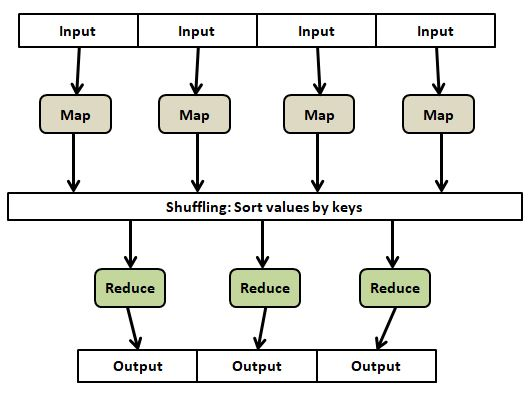
\includegraphics[scale=1.00]{Mapreduce}
	\caption{An illustration of MapReduce programming model based on \cite{elsayed2008pairwise}}
	\label{fig: Mapreduce}
\end{figure}

\par To define a function by a user, the following are the signatures provided as an abstraction by the MapReduce 
\cite{elsayed2008pairwise}:

\[Map: (Key1,Value1) \implies list(Key2,Value2)\]
\[Reduce: (Key2,list(Value2)) \implies list(Key3,Value3)\]


To process big data across multiple clusters based on the Google's MapReduce, Apache developed an open source framework referred as Apache Hadoop. The framework is developed for processing distributed and scalable computations. Hadoop Distributed File System (HDFS), Hadoop common, Hadoop YARN and Hadoop MapReduce are the major components offered by the Hadoop and are discussed in the following \cite{website:hadoop}:

\begin{itemize}
\item Hadoop Common: This module helps in the startup of the Hadoop by running the configuration scripts. Also, this module includes abstraction for operating systems and Java libraries.

\item Hadoop YARN: This module is responsible for scheduling of job tasks and management of resources across clusters. The management of resources is processed through node managers and resource managers by YARN. YARN abbreviates to Yet Another Resource Negotiator. 

\item Hadoop MapReduce: This component offers MapReduce programming model on YARN clusters for parallel processing of data sets of large scale.

\item Hadoop Distributed File System (HDFS): This component offers to store huge voluminous dataset through the distributed file system in a cluster. The advantage of this component is it to make sure that data is accessible by all nodes in the cluster. Hence, is suitable for large scale applications.

\end{itemize}


\textbf{Limitations}
\par Though MapReduce has many advantages for parallel processing of big data but shows inefficiency in performing computations for applications that use iterative algorithms as well as for interactive applications. Some of the reasons are stated below \cite{Jonnalagadda2016}:

\begin{itemize}
\item Because of writing and reading of inputs/outputs to and from disks, serialization, and replication, the data sharing between tasks are time consuming. Hence most of the applications allocate greater time in read-write operations.

\item The applications that use iterative algorithms often need data to be reused multiple times. When an iterative application is processed on MapReduce, the intermediate results in MapReduce programming model writes to disks on every iteration thereby causing an I/O communication overhead which can be seen in \ref{fig: iteration}.
\end{itemize}

\begin{figure}[htbp]
	\centering
		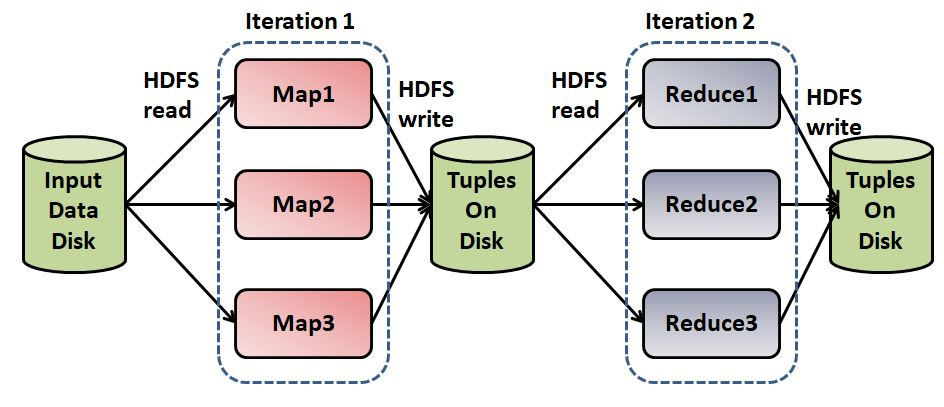
\includegraphics[scale=0.60]{Iteration}
	\caption{An Example of iteration process in MapReduce \cite{Jonnalagadda2016} }
	\label{fig: iteration}
\end{figure}



\section{Apache Spark}
\label{section: apache spark}
This thesis uses the Apache Spark framework to implement parallel processing of a large set of documents. Hence, this section provides the bedrock information about Apache Spark.

\par Apache Spark, an open source cluster computation engine for processing and analyzing huge voluminous data commonly referred as big data. It was initially developed by Matei Zaharia in 2009 at UC Berkeley's AMPLab \cite{Jonnalagadda2016}. It is a unified framework to support a variety of workloads including streaming, batch processing, iterative algorithms and interactive queries \cite{karau2015learning}. One of the fundamental highlights Spark offers for speed is the capacity to run computations in-memory. Another being tight-integration with other big data tools, accessibility of application programming interfaces (APIs) in various programming languages like Scala, Java, Python and R \cite{karau2015learning}. 

\par MapReduce and many of its versions use an acyclic data flow model and have been efficient in performing voluminous data-intensive applications on commodity clusters. But they are not appropriate for interactive data analytics, machine learning applications which uses algorithms that are iterative in nature and requires functional dataset to be reused across multiple parallel operations \cite{zaharia2010spark}. On surveying these drawbacks, researchers Matei Zaharia, Mosharaf Chowdhury, Michael J. Franklin, Scott Shenker and Ion Stoica presented a framework named Spark.
 
 
\par Spark works on in-memory cluster computation while preserving the properties such as scalability and fault tolerance of MapReduce \cite{zaharia2010spark}. Rather than loading of data from disk, Spark facilitates the machines to cache intermediate results and data in memory on each iteration. Thus, offering more space for efficiency in iterative computations and is appropriate for substantial scale machine learning applications \cite{bao2016large}.

\par  The primary idea on which Spark was build for distributed shared memory abstraction is adverted as Resilient Distributed Datasets (RDDs)  \cite{Zaharia2012}. In \ref{Spark Core}, the concept of RDDs is discussed in detail. 


\subsection{Traits of Spark}
Other traits apart from in-memory cluster computations of Spark are discussed in this section.
\begin{itemize}
\item \textbf{Swift Processing:} As spark benefits from in-memory caching, the computational performance of Spark in Hadoop clusters is 100 times swifter if run in memory and 10 times if run on disk when compared to Hadoop MapReduce\cite{spark:website}. For an identical application, the difference in runtime performance between Spark and Hadoop is illustrated in \ref{fig:runtime}

\begin{figure}[htbp]
	\centering
		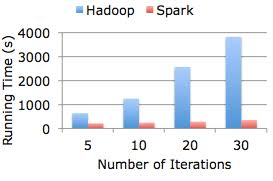
\includegraphics[scale=1.00]{runtime}
	\caption{Total runtime performance of logistic regression in Spark and Hadoop \cite{spark:website} }
	\label{fig:runtime}
\end{figure}

\item \textbf{State-of-the-art analytics:} Spark is not only limited to map and reduce functions. For advanced analytics,  Spark's support is extended to Machine learning algorithms, SQL queries, Graph algorithms, and Streaming data \cite{ranjani2016spark}. Additionally, Spark provides its users the functionality to combine any of these libraries into a singular process workflows to perform complex computations \cite{Jonnalagadda2016}.
\end{itemize}

\newpage
\subsection{Ecosystem}
As shown in \vref{fig:ecosystem}, Spark ecosystem consists of four prime components built on top of Spark's core and are discussed below in detail.

\begin{figure}[htbp]
	\centering
		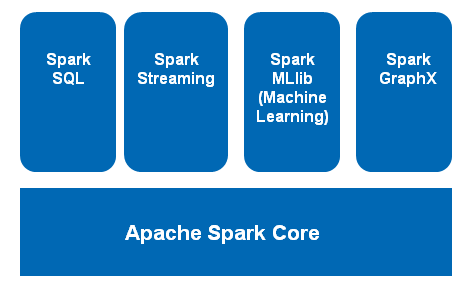
\includegraphics[scale=1.00]{Spark_ecosystem}
	\caption{Apache Spark Ecosystem \cite{spark:website}}
	\label{fig:ecosystem}
\end{figure}


\subsubsection{Spark Core}
\label{Spark Core}
Spark core is the heart to the APIs that exemplify Resilient Distributed Datasets (RDDs). The RDD API provides a programming interface for substantial scale data processing. These APIs can be programmed in Scala, Java, Python, and R. Besides, Spark Core is responsible for shuffling and scheduling of tasks, memory management between nodes in a cluster. Furthermore, libraries on top of the Spark Core handle diverse workloads. By optimizing the Spark Core, these libraries can be optimized.

\par  Resilient Distributed Datasets (RDD) are primarily responsible for data abstraction in Spark Core and are discussed in detail in the succeeding section. 

\textbf{Resilient Distributed Datasets}
\par Resilient Distributed Dataset (RDD) is a large set of immutable objects that are distributed parallel across nodes in a cluster \cite{Zaharia2012}. Spark offers RDDs, Accumulators, and broadcast variables as major data abstractions to its users to program clusters and two shared variables which are of restricted type \cite{zaharia2010spark}. The RDD is constructed with the assistance from Direct Acyclic Graph (DAG) which is a tree lineage. This lineage helps RDDs evade from data replication by keeping track of its transformations. As a result, RDDs are fault tolerant and they benefit from re-computation of data when one of its partitions is lost due to failure \cite{salloum2016big}.

\par RDDs can be created in Spark by two following ways \cite{karau2015learning,spark:website}:
\begin{enumerate}
\item By accessing data from external sources
\item By caching or persisting from already available RDDs
\end{enumerate}


\begin{figure}[htbp]
	\centering
		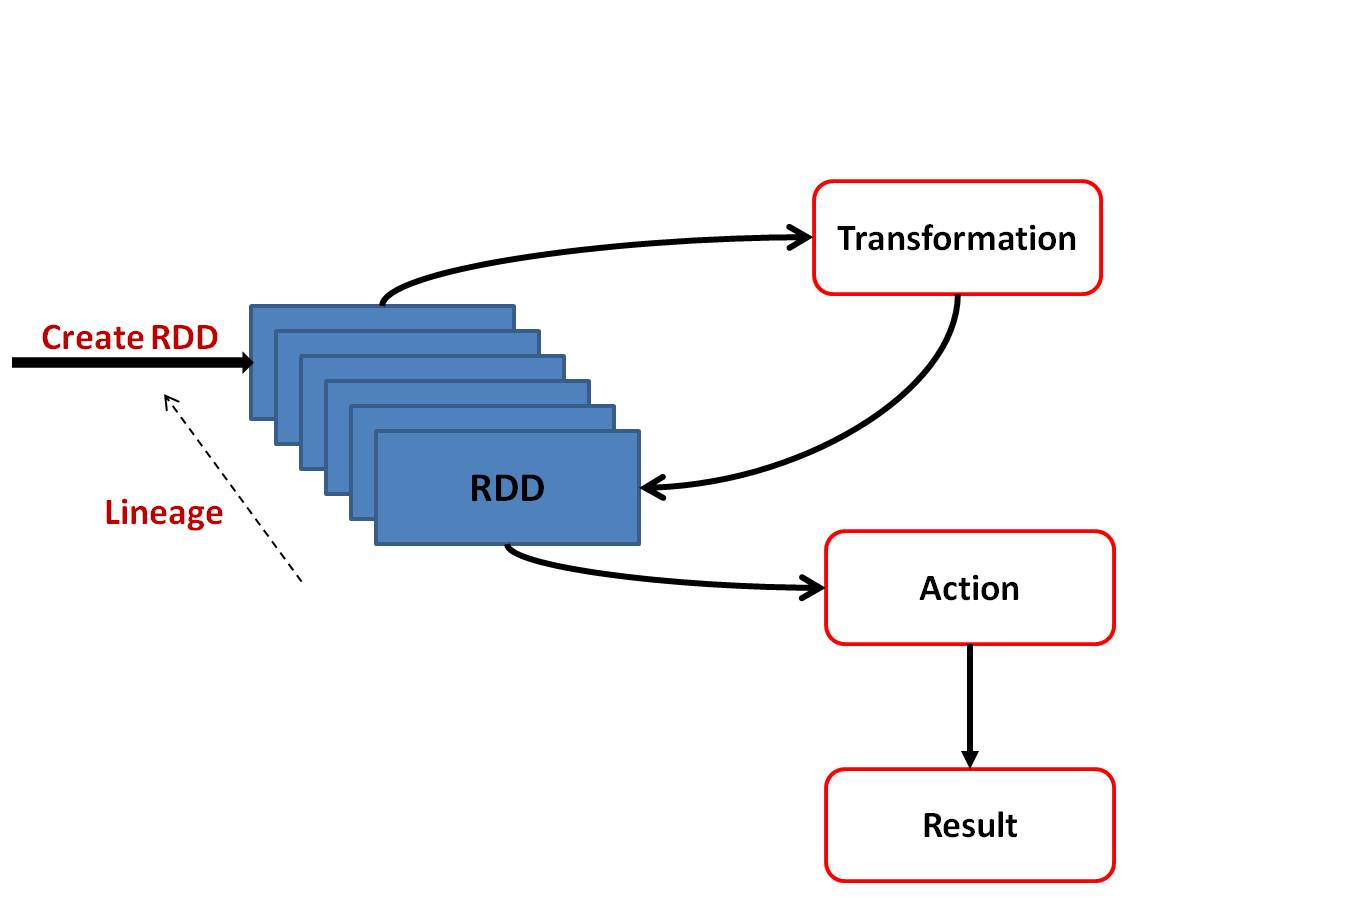
\includegraphics[scale=0.60]{RDD}
	\caption{Workflow of RDDs}
	\label{fig:RDDs workflow}
\end{figure}

\par As shown in \ref{fig:RDDs workflow}, there are mainly two types of operations namely Transformations and Actions that can be performed on RDDs \cite{zaharia2010spark,spark:website,karau2015learning}. 

\textit{Transformations:} From existing RDDs, a new transformed RDD is created using this operation. When a transformation operations are applied on RDDs, RDDs do not transform immediately until an action is called upon them. But instead, Spark remembers the metadata of transformations to be applied. Hence in Spark, these operations are termed as lazy evaluations. A bunch of these transformations operate element-wise (one element at a time) but not in every case \cite{karau2015learning}.

\par Part of the transformation operators usually used in Spark includes \cite{spark:website}:

\begin{itemize}
\item \textit{filter():} This operator is used when required to return selected elements from the previous dataframe through a function m.
\item \textit{map():} This operator returns a distinct dataframe by passing the function m to each element in the dataset.
\item \par\textit{join():} This operator is used to combine two dataframes with a join condition and returns a new dataframe. 
\item \textit{repartition():} This operator is used to randomly reshuffle the data partitions either to increased partitions by creating or fewer partitions by deleting across all the nodes in a cluster.
\end{itemize}

\textit{Actions:} After applying action operator on the RDDs, the resulting transformation returns the values to the driver program \cite{spark:website}.
\newline
\par Some member operators belong to this type include \cite{spark:website}: 

\begin{itemize}
\item \textit{collect():} Returns entire elements of a dataframe in the form of array to the driver program.
\item \textit{count():} This operator counts the total number of elements available in the dataframe.
\item \textit{take(m):} This operator returns the first m elements from the dataframe.
\item \textit{first():} This operator returns the first element in the dataframe.
\item \textit{reduce():} This operator merges elements in the dataframe with specified function m.
\end{itemize}


\textbf{Broadcast Variables} 
\par As discussed earlier in spark, Broadcast Variables comes under the hood of Shared Variables which are used for specific purpose. As a rule, the functions like map, reduce are executed by copying every variable associated with the function on all nodes in a cluster. But any update on these variables from any node will not be transmitted back to the driver program \cite{spark:website}.

\par Instead of copying all the variables associated with the task, Broadcast variables are cached to all nodes in a cluster irrespective of their association. Use of Broadcast variables is advantageous when there is a need for the huge volume of input dataset to be cached on all nodes. With broadcast algorithms, Spark can efficiently distribute the broadcast variables across all the nodes and also minimize the communication between nodes \cite{spark:website}.

\subsubsection{Spark SQL}

\par Spark SQL is another rich library built on top of Spark Core. Spark SQL is developed to perform relational database related query operations on RDDs but limited to structured and semi-structured data. Any data is said to be structured if every record in a dataset was defined with a schema. Similarly, if the schema can be defined explicitly then the data is said to be semi-structured. Spark supports to read data from formats like Hive tables, JSON, Parquet. Using Spark SQL on big data, all the relational SQL queries can be performed in parallel \cite{spark:website}. 

\par The fundamental aspect which makes Spark SQL differ from Spark RDD API is the interface offered by Spark SQL. This interface provides additional information related to the data structure alongside computations to Spark. With this additional information, Spark SQL can perform further optimizations.


\par Moreover, Spark SQL is now capable of integrating SQL queries and procedural code in one single application. Thus, with this integration Spark can perform complex analytics. For instance, processing of machine learning algorithms and graph algorithms on diverse big data applications. Spark SQL achieved this intermix by two models namely DataFrame API and optimizer titled Catalyst \cite{armbrust2015spark}.

\par In the consecutive sections, DataFrames are discussed in detail.

\textbf{DataFrames}

\begin{figure}[htbp]
	\centering
		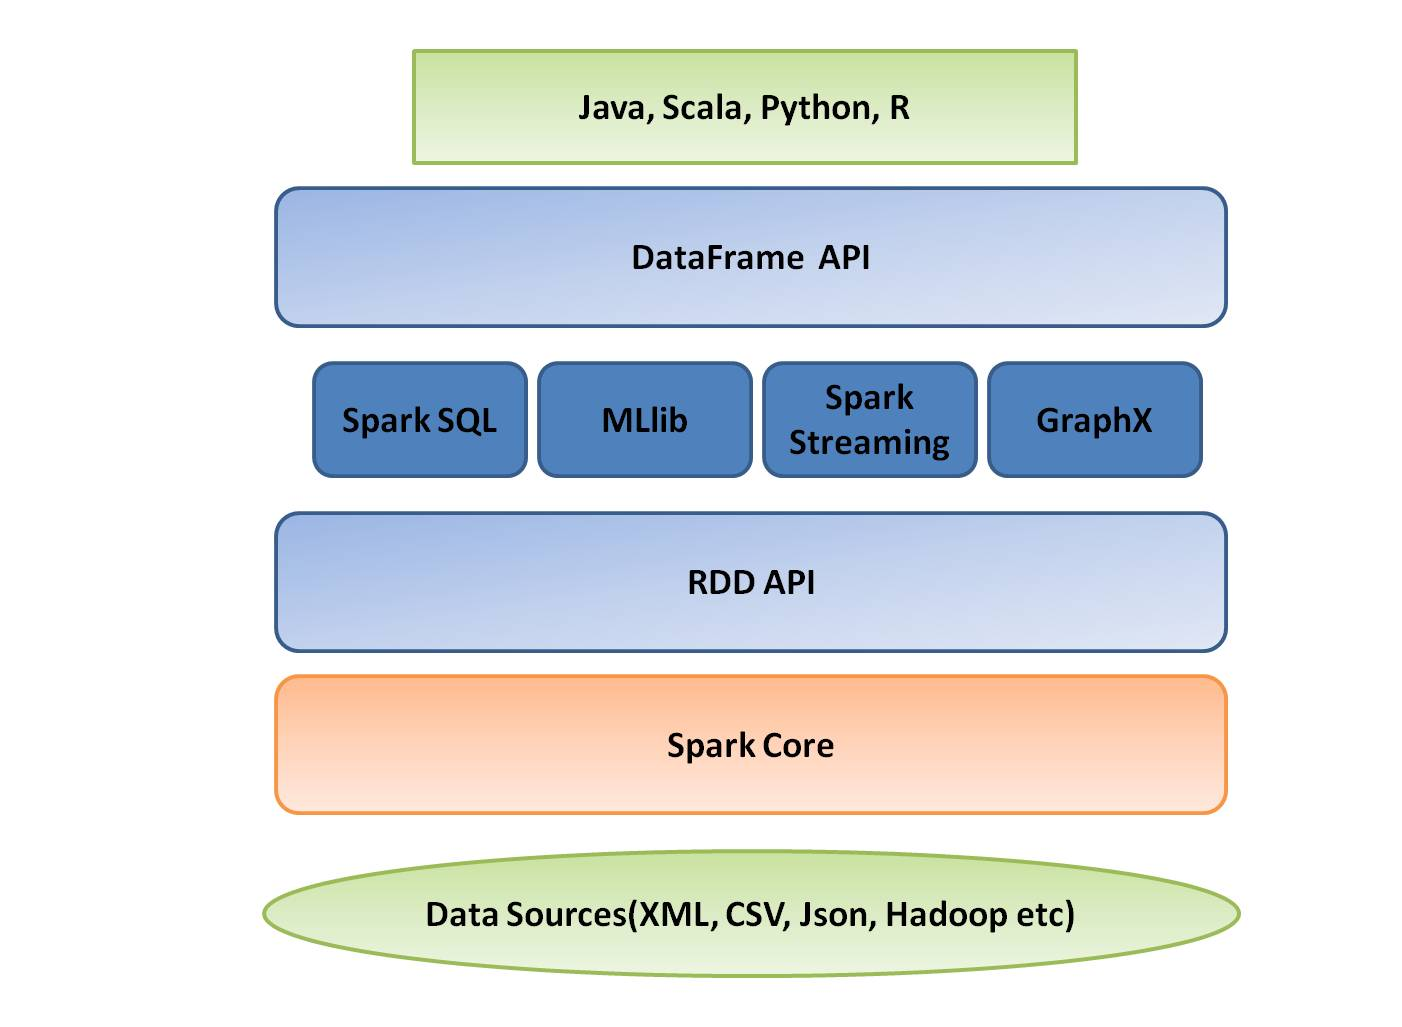
\includegraphics[scale=0.60]{DataFrames_API}
	\caption{DataFrame API in Spark Ecosystem }
	\label{fig: DataFrame API}
\end{figure}

\par DataFrames are generally known abstractions of tables in Python and R. For Structured Data and semi-structured data, the DataFrame API provides a high level abstraction of the Spark SQL. Similar to RDDs, DataFrames are also large sets of distributed data collection but with organized named columns as well as maintain a record of their schema for increased optimizations. Scala, R, Python, and Java support DataFrame API and illustrated in \ref{fig: DataFrame API}. DataFrames can be constructed with multiple sources ranging from existing RDDs to external databases. In Python, the DataFrame on a conceptual level is identical to a relational database table \cite{spark:website}.


\begin{figure}[htbp]
	\centering
		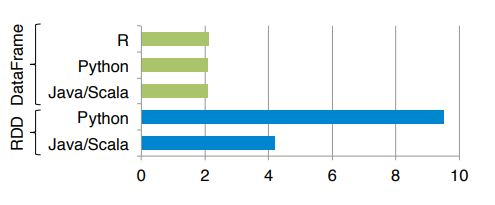
\includegraphics[scale=1.00]{RDD_vs_Dataframe}
	\caption{Difference in Execution time (Seconds) taken by RDD API and DataFrame API for a aggregation query using distinct programming languages \cite{armbrust2015scaling} }
	\label{fig: RDDvsDataFrame}
\end{figure}

\par The compelling feature of the DataFrame is storage of data in a columnar fashion which is much more consistent than Java/Python objects. As shown in \ref{fig: RDDvsDataFrame}, DataFrames can compute multiple aggregations efficiently using a single SQL statement when compared to Spark functional API irrespective of the programming language \cite{armbrust2015spark}. Within Spark applications, DataFrame APIs provide functional integrations with Spark SQL to other libraries. As a result, DataFrames are now prime representations to Spark's ML Pipeline API, GraphX and GraphFrames \cite{karau2015learning}.

\par Antithetical to Spark APIs, DataFrames hold relational operations as domain-specific language (DSL) expressions which then translate to abstract syntax trees (AST) and send to Catalyst optimizer to ensure optimization. This functionality enabled DataFrames to compute efficiently and conveniently than RDD API. Furthermore,  DataFrames in Spark is lazily evaluated which means there will be no execution of the logical plan until the user calls an action. The logical plan is stored as an individual DataFrame object for computations on dataset \cite{armbrust2015spark}. Apart from these, DataFrames not only restricted to use of its built-in functions but also supports User Defined Functions (UDFs) in which user can define own functionality to their applications.

\par The DataFrame API provides a variety of operations that can be performed on a DataFrame. Segment of these operators like alias(), count(), cache(), withColumn(), repartition() are used in our application and are described below \cite{spark:website}:

\textit{alias():} With this operator, a new DataFrame can be created by replicating the original DataFrame.

\textit{cache():} With the use of this operator, DataFrame will be cached to in-memory.

\textit{count():} Count operator counts the total number of rows that a DataFrame consists and returns the value.

\textit{repartition():} With this operator, a DataFrame can be equally partitioned into \textit{p} partitions.

\textit{withColumn():} Either by creating a new column or replacing a column can be performed to the existing DataFrame by use of this operator. For instance, if a DataFrame has two columns (\textit{Col a, Col b}) then a third column (\textit{Col c}) can be added to it by invoking this operator.

\subsubsection{Spark Machine Learning (MLlib)}

\par To process large scale datasets that require iterative algorithms in a distributed environment, Spark provides a high level machine learning API build on top of Spark Core as illustrated in \ref{fig:ecosystem}. As Spark benefits from in-memory computations, it makes convenient for iterative machine learning applications because any enhancements applied to Spark Core enhances the performance in upper-level libraries without explicit changes to the upper-level libraries. Hence improved enhancements in Spark MLlib with Spark's integration.

\begin{figure}[htbp]
	\centering
		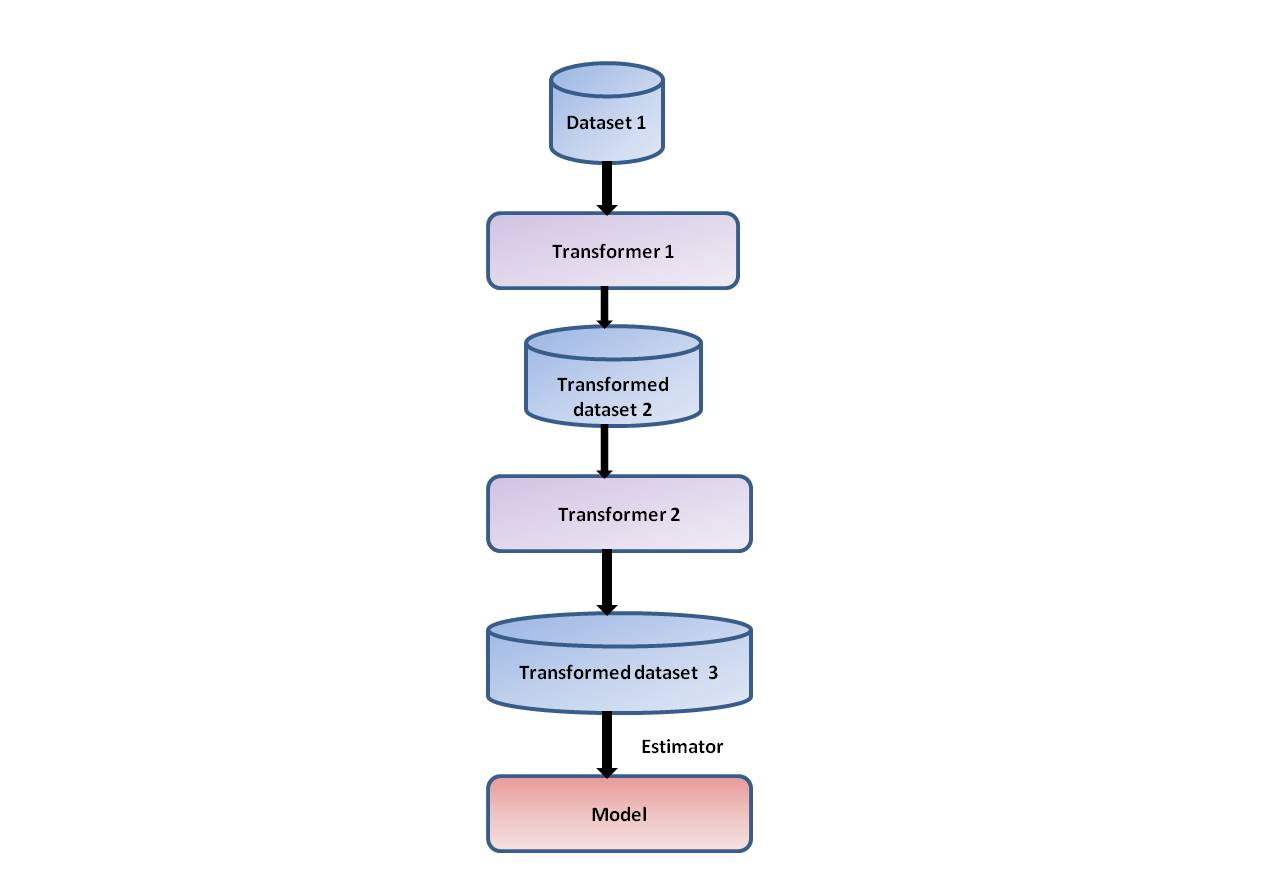
\includegraphics[scale=0.75]{pipeline}
	\caption{An example machine learning workflow with transformers and estimators}
	\label{fig: pipeline}
\end{figure}

\par Machine learning in Spark is divided into mllib and ml packages. The package mllib is built on top of RDDs whereas package ml is built on top of DataFrames. According to \cite{spark:website}, Spark now uses DataFrame-based API as prime machine learning API as the DataFrames are advantageous in many scenarios than RDDs including its optimized computations, simplified data integration to Spark SQL. The conversion of DataFrame to RDD and vice-versa can be applied to all algorithms of the Spark's Mllib by swapping conveniently from ml to mllib.


\par Spark's machine learning library comes with a variety of machine learning techniques include  Clustering, Transformers, Extractors, Classification, Clustering, Dimensionality Reduction. Like Spark Core, Spark Mllib also supports Scala, Java and Python programming languages to develop scalable machine learning algorithms. Additionally, it also supports a wide range of statistics, evaluation methods and linear algebra that are generally required for general machine learning applications for purpose of analytics \cite{meng2016mllib}.



\par Generally, many of the machine learning applications process data in sequential stages that involve preprocessing to validation stages which are commonly referred to a pipeline. Spark MLlib provides the pipeline functionality through ml API to construct efficient data workflows in a simplified manner. Each stage in the ml pipeline contains Transformers and Estimators. Transformer receives the input dataset, performs a transformation technique that is chosen and the output of the transformed data is fed into next stages of ml pipeline. Usually, these transformers in machine learning are used for feature extractions from input dataset. Likewise, an estimator is used for producing a model with the transformed data. An estimator is always followed by a transformer and is illustrated in \ref{fig: pipeline}. Pipelines are useful to configure any number of stages for a large scale machine learning applications \cite{website:databricks}. 

\par From \ref{fig: pipeline}, we can observe that the size of the dataset is increasing after it is fed into transformers. This is because when a transformer transforms data, a new column is generated as an output column for the transformation technique applied and then finally a model is produced by invoking the estimator.


\textbf{Vectors}

\par Under the mllib package, Spark represents two vector classes called Sparse Vectors and Dense Vectors for the purpose of vector related computation processing. Sparse Vectors stores only non-zero values to an array object where as Dense Vector stores all the values in an array of objects and can be used for mathematical calculations with other array objects. But, Spark allows Dense Vectors to store values as numpy floating object which translates to that even if an integer value is passed to the vector the resulting vector would be of type float. With the help of RDD transformations, these dense vectors can be distributed to all other RDDs as these objects are locally exist intrinsically \cite{website:densevectors} \cite{website:documentation}.



\subsubsection{Spark Streaming}

To process the huge amount of data in real-time, Spark Streaming library was developed as an extension to Spark Core API. A programming model called discretized streams or (DStreams) is the primary abstraction for Spark Streaming. The RDDs arranged in series represent DStreams. With a wide range of input streams namely Twitter, Kafka, Flume and etc DStreams can be created and then can be transformed to databases. Moreover, DStreams can also be created by other DStreams. Scala, Java and Python APIs are supported by Spark Streaming. Every RDD created by DStream contains the data with a specific time interval which can be referred as micro batching. With Spark Streaming, a streaming application that requires scalability, as well as fault tolerance as factors can be built \cite{spark:website}.

\subsubsection{Spark GraphX}
 For distributed environments, Spark offers GraphX library to process graph based data computations. 

As our application does not require Spark GraphX and Spark Streaming, We have briefly discussed them.

\subsubsection{Management of Clusters}
\label{section: management of clusters}
Spark requires cluster managers to access data from external sources encompassing Cassandra, HBase, HDFS \cite{Jonnalagadda2016}. Spark Core is built on top of cluster managers to facilitate this purpose. The job of the cluster manager is to allocate and supervise available cluster resources between spark applications. Spark not only runs on its standalone cluster manager but also integrates with distinct cluster managers accommodating Hadoop YARN, Apache Mesos, and Amazon EC2 \cite{karau2015learning}.


\par Spark application can be submitted by either local mode or cluster mode. To process the huge voluminous data, cluster mode is used. On the other hand, a local mode is used for the purpose of testing the application. The cluster mode functions in master/slave architecture where the slaves are connected in a distributed environment. The slaves are also called as workers. When an application is launched in cluster mode, then the master node divides the program execution into smaller chunks and are distributed across the workers.

\section{Related Work}
\label{section: Related work}
In this section, previously carried out implementations in the area of document matching as well as Latent Dirichlet Allocation are discussed. Various concepts exist to improve the execution time in the field of LDA algorithms with parallel computational processing.  \ref{subsection: mpi based} and \ref{subsection: Mapreduce based} provides information on such implementations which focuses primarily on improving the LDA algorithms for parallel environments. Only few relevant concepts that we think mostly related to this thesis are discussed although many implementations exist.


\subsection{MPI Based Implementation}
\label{subsection: mpi based}
MPI abbreviates to Message Passing Interface. MPI uses message passing programming model. MPI benefit from Universality, Expressivity, and Ease of debugging. MPI is most widely used programming model to implement algorithms using parallel processing. MPI is not a language but a library provided to implement parallel computing applications \cite{gropp1999using}. The paper \cite{wang2009plda} discuss the parallel implementation of the Latent Dirichlet Allocation (LDA) using MPI programming model. The implementation uses AllReduce algorithm in assistance with the MPI. The major focus of the implementation was to parallelize the process of topic assignment of the documents in the huge collection thereby achieving the scalability. Finally, the authors measured the speed up and execution time of the implementation. The authors also made available the source code of MPI implementation under Apache open source License.

\subsection{MapReduce Based Implementation}
\label{subsection: Mapreduce based}

In the same paper \cite{wang2009plda}, the authors discusses the implementation of LDA using MapReduce programming model. In \ref{section: Mapreduce}, the core concepts regarding the MapReduce programming model along with its advantages and limitations are discussed in detail. The implementation processes the huge volume of data by dividing and distributing them across multiple workers in a cluster. As discussed in \ref{section: Mapreduce}, the MapReduce programming model consists of two stages namely map and reduce. The authors defined the map phase as sampling phase where the topic assignment of the documents using Gibbs algorithm takes place. Then, the reduce phase receives these topic assignments and update the model. The implemented application is then measured for Speedup and execution time. The two datasets namely Wikipedia and Forum dataset are used for evaluating the speedup performance. A comparison was made between the MPI based and MapReduce based implementations where the implementation based on the MPI overrules the MapReduce based implementations and the reasons are discussed.


\par The work in  \cite{elsayed2008pairwise} discusses the problems associated with the computations of pairwise document matching based on their similarity within a set of documents in huge volume. The author presented an implementation using MapReduce programming model as a solution to the above addressed problem. The chief purpose of the paper focuses on processing the huge set of documents by representing them as a bag of words irrespective of the order along with their term weights. The term weights provide information of the term importance in any document. The implementation processes indexing of documents in Map phase and computes pairwise similarity in reduce phase. The implementation was evaluated on cluster consists of 20 machines and calculated the runtime performance. For evaluation, the AQUAINT-2 dataset is used. 

%- Allgemeine Wissensgrundlagen des Fachgebiets
%- Spezielle Grundlagen, die für das Verständnis erforderlich sind
%- Rahmenbedingungen für die Arbeit
%- Ausführungen zum Stand des Wissens / der Technik
%Als Leitprinzip gilt: Nur Informationen erwähnen, die
%- später benötigt werden,
%- notwendig sind, um die Arbeit oder ihre Motivation zu verstehen
%Das heißt insbesondere,
%- keine Inhalte aus Lehrbüchern, außer
%- diese werden benötigt, um Problemstellung oder Lösungsweg zu definieren.
